\section{\textit{Embeddings}}

gesnim word2vec model

Parameters:
\begin{itemize}
    \item Embedding Size:
    
    \item Window:
    
    \item Min Count:
    
    \item SG:
    
    \item Negative:
\end{itemize}

\subsection{2D Plots}

PCA

\subsubsection{Simpsons Dataset}

\begin{figure}[H]

\centering
\begin{minipage}{0.47\textwidth}
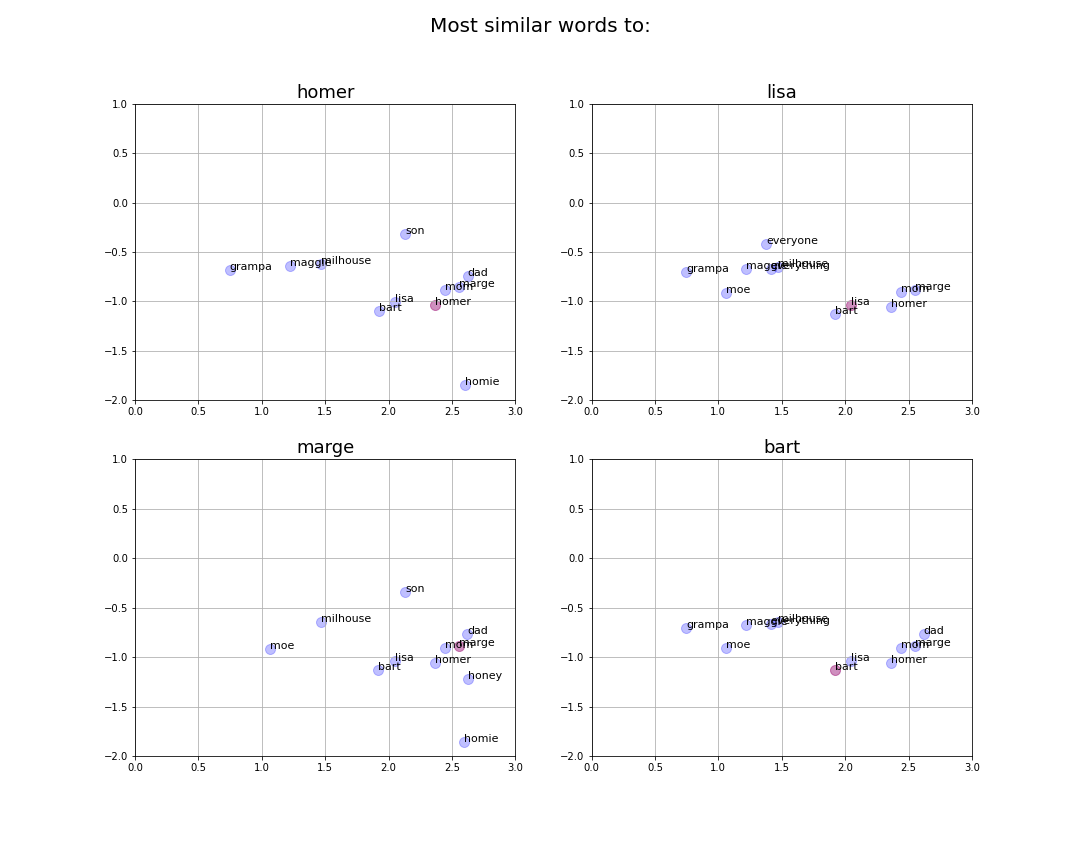
\includegraphics[trim=4.2cm 3cm 3.7cm 2.7cm, clip=true, width=\textwidth]{results/embeddings/simpsons_similar_15.png}
\caption*{a) DIM = 15}
\end{minipage}\hfill
\begin{minipage}{0.47\textwidth}
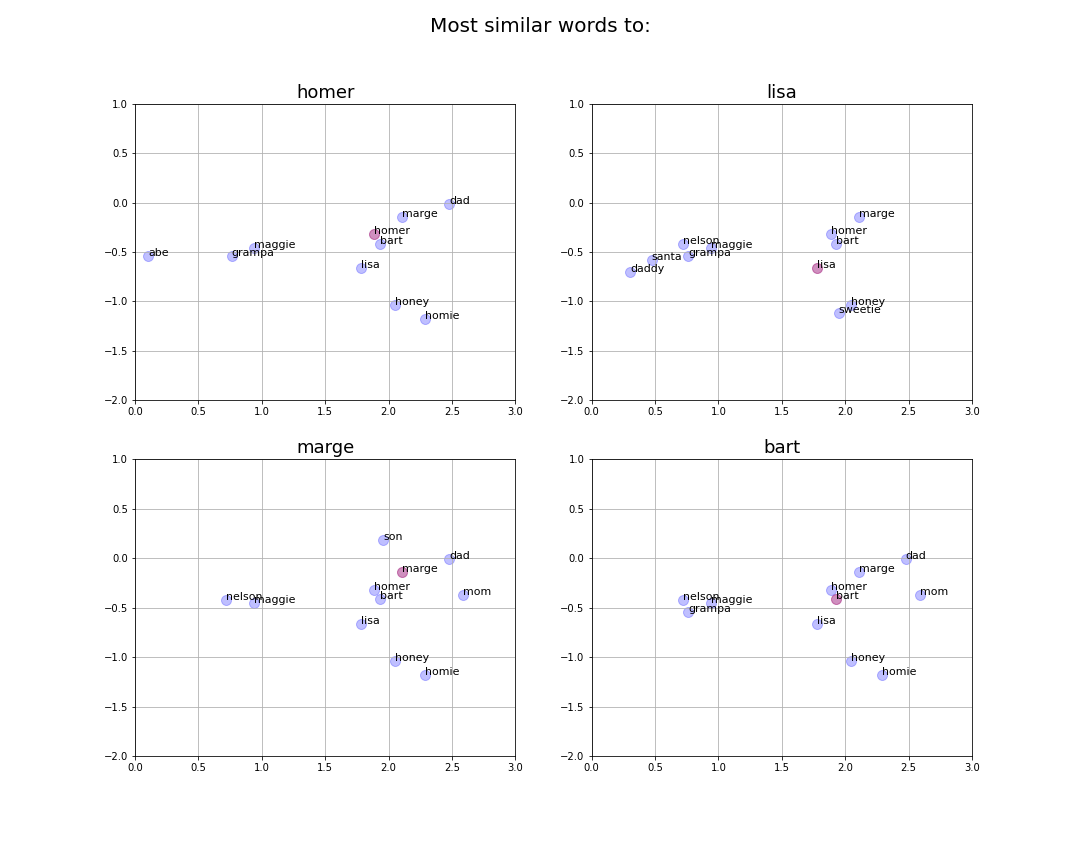
\includegraphics[trim=4.2cm 3cm 3.7cm 2.7cm, clip=true, width=\textwidth]{results/embeddings/simpsons_similar_75.png}
\caption*{b) DIM = 75}
\end{minipage}\par
\vskip\floatsep% normal separation between figures
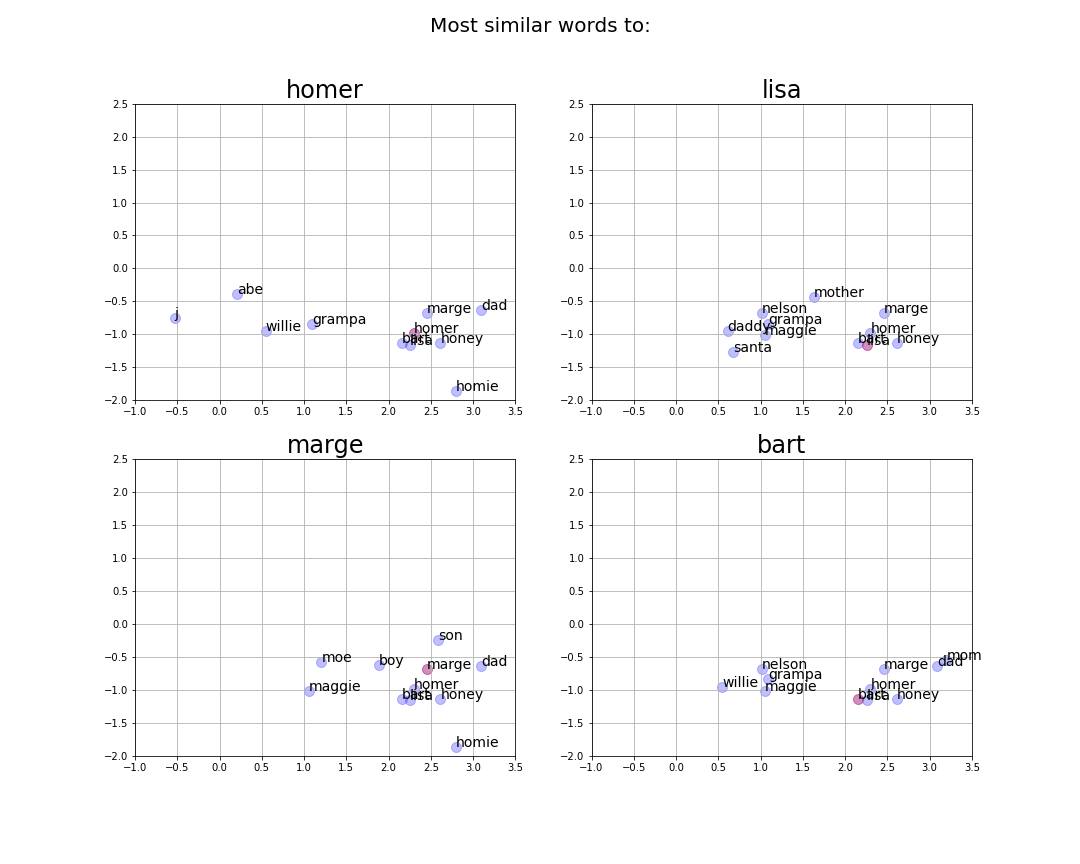
\includegraphics[trim=4.2cm 3cm 3.7cm 2.7cm, clip=true, width=0.45\textwidth]{results/embeddings/simpsons_similar_150.png}
\caption*{c) DIM = 150}
\caption{\textit{Embeddings} de los personajes principales de los \textbf{\textit{Simpsons}} y los términos más similares proyectados en un plano 2D para distintos tamaño de \textit{embedding}}
\label{fig:simpsons_sim_words}

\end{figure}


\subsubsection{Friends Dataset}

\begin{figure}[H]

\centering
\begin{minipage}{0.47\textwidth}
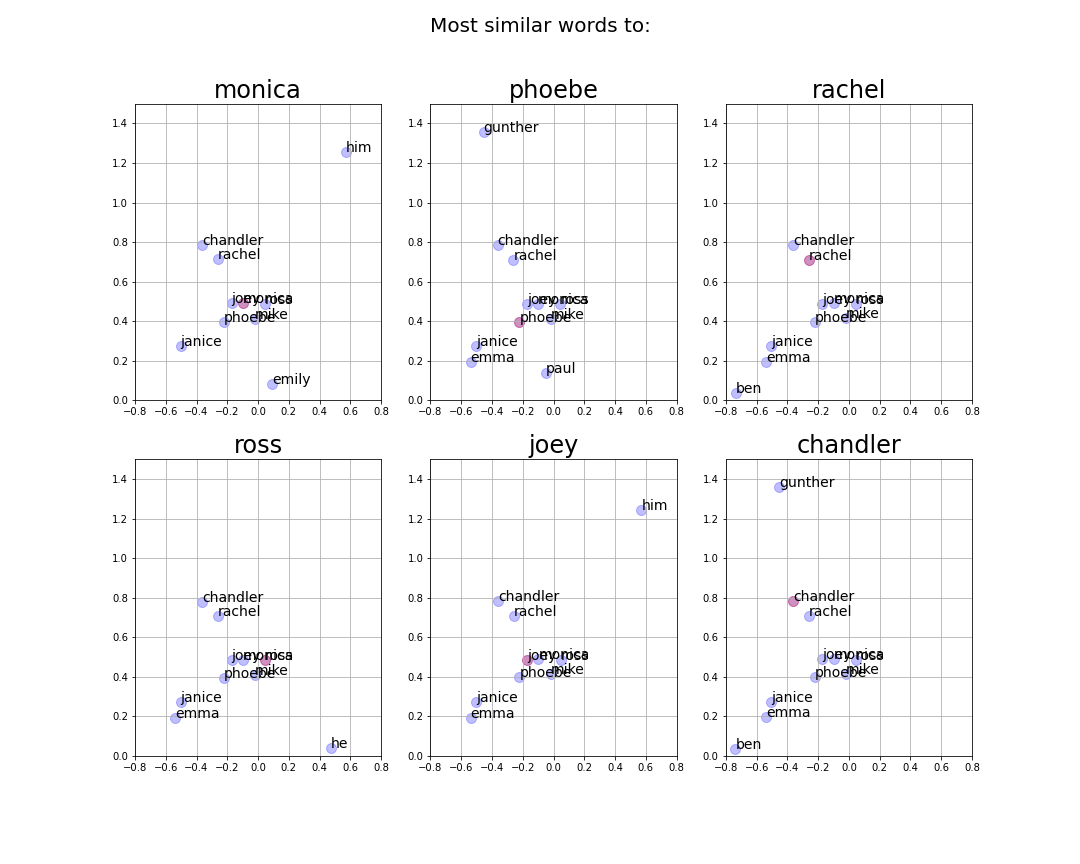
\includegraphics[trim=4.2cm 3cm 3.7cm 2.7cm, clip=true, width=\textwidth]{results/embeddings/friends_similar_15.png}
\caption*{a) DIM = 15}
\end{minipage}\hfill
\begin{minipage}{0.47\textwidth}
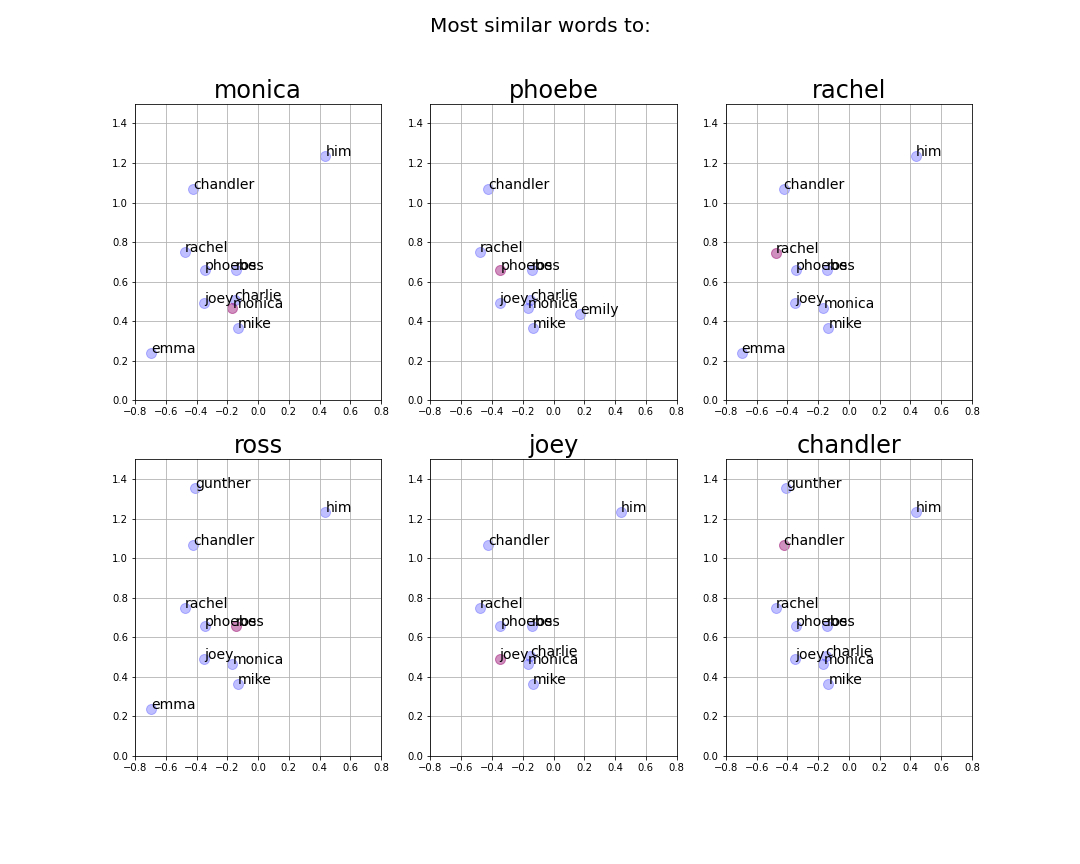
\includegraphics[trim=4.2cm 3cm 3.7cm 2.7cm, clip=true, width=\textwidth]{results/embeddings/friends_similar_75.png}
\caption*{b) DIM = 75}
\end{minipage}\par
\vskip\floatsep% normal separation between figures
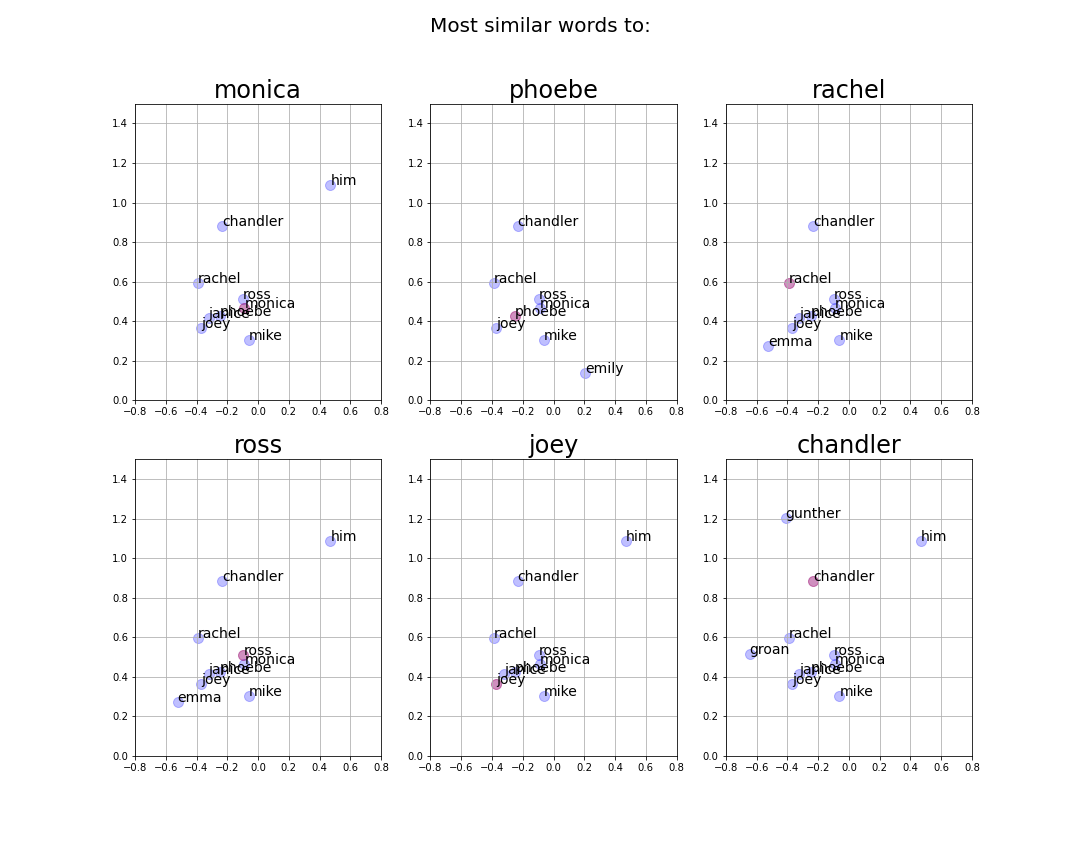
\includegraphics[trim=4.2cm 3cm 3.7cm 2.7cm, clip=true, width=0.45\textwidth]{results/embeddings/friends_similar_150.png}
\caption*{c) DIM = 150}
\caption{\textit{Embeddings} de los personajes principales de \textbf{\textit{Friends}} y los términos más similares proyectados en un plano 2D para distintos tamaño de embedding}
\label{fig:friends_sim_words}

\end{figure}

\subsection{Interesting Relations}
\begin{itemize}
    \item Similaridad
    
    \item Analogía 
    
    \item Coincidencia (\textit{doesn't match})
\end{itemize}

\subsubsection{Simpsons Dataset}

\begin{figure}[H]
    \centering
    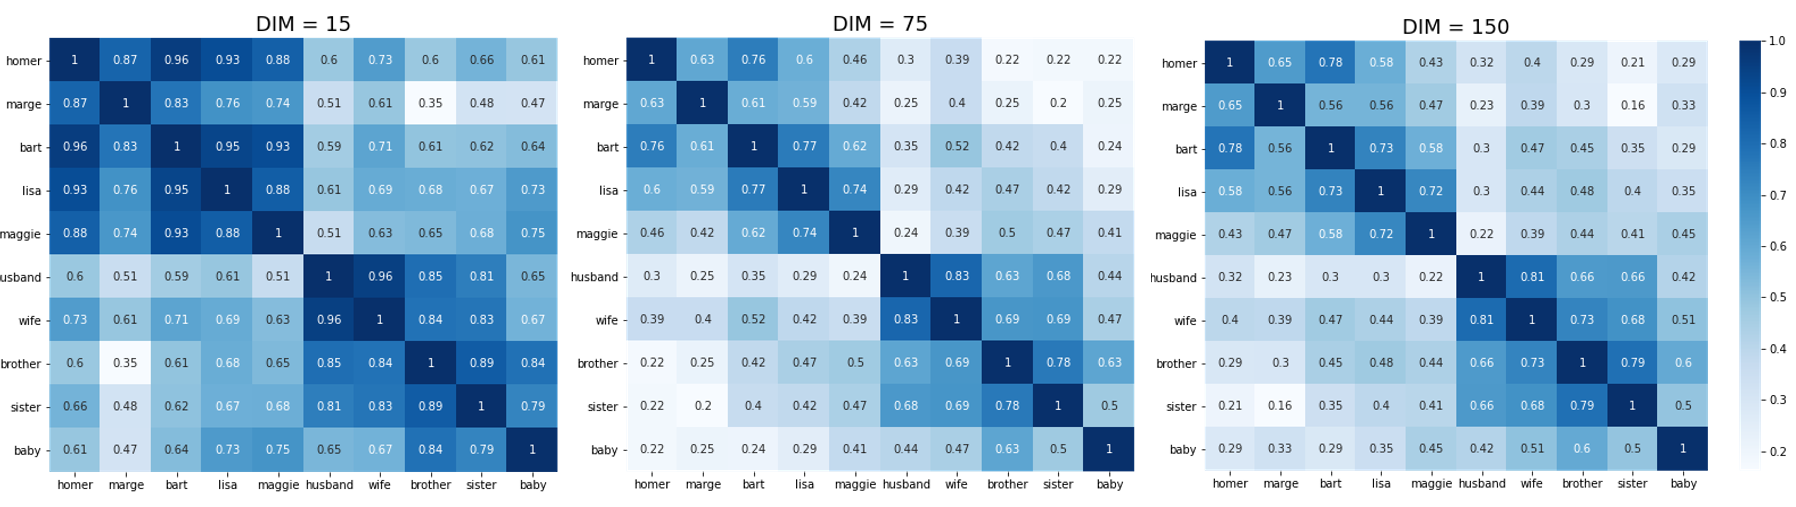
\includegraphics[width=\textwidth]{doc/images/simpsons_sim_matrix.png}
    \caption{Caption}
    \label{fig:simpsons_sim_matrix}
\end{figure}

\subsubsection{Friends Dataset}

\begin{figure}[H]
    \centering
    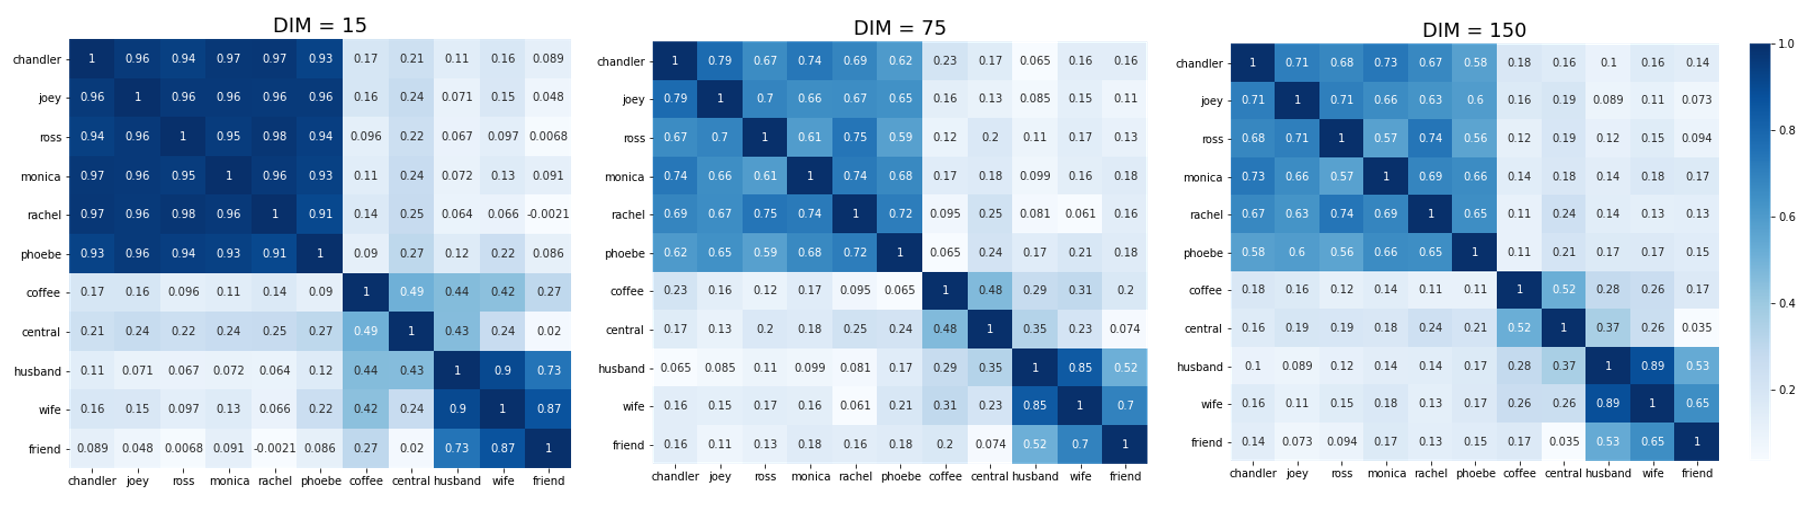
\includegraphics[width=\textwidth]{doc/images/friends_sim_matrix.png}
    \caption{Caption}
    \label{fig:friends_sim_matrix}
\end{figure}

\newpage